%:
\documentclass[9pt]{scrartcl}
\usepackage{amsmath}
\usepackage[forpaper,nopopontsals,nosolutions]{eqexam}
\usepackage{chemformula}
\usepackage[version=4]{mhchem}
\usepackage[utf8]{inputenc}
\usepackage[T1]{fontenc}
\usepackage{booktabs}
\usepackage{setspace}
\usepackage[spanish]{babel} 
\usepackage[left=2cm,top=0.35cm,right=2.5cm,bottom=1cm]{geometry}
\usepackage{varwidth}
\spanishdecimal{,}
\pointLabel{punto}
\pointsLabel{puntos}
\ptLabel{pt.}            % singular form
\ptsLabel{{pts.}}
\eachLabel{\tiny{apdo.}}
\renewcommand\itemPTsTxt[1]{{\footnotesize $#1$ pts}}
\usepackage[version-1-compatibility]{siunitx}
%\usepackage{times}
%\usepackage{newcent}
\usepackage{palatino}
%\usepackage{bookman}
%%%%%%%%%%%%%%%%%%%%%%%%%%%%%%%%%%%%%%%%%%%%%%%%%
%%%%%%%%%%%%%%%%%%%%%%%%%%%%%%%
% %%                    zona de unidades                 %%%%%%
%%%%%%%%%%%%%%%%%%%%%%%%%%%%%%%
%%%%%%%%%%%%%%%%%%%%%%%%%%%%%%%

\usepackage{siunitx}
\sisetup{inter-unit-product = \ensuremath{{}\cdot{}}}
\sisetup{quotient-mode=fraction}
\sisetup{per-mode=fraction}
\sisetup{exponent-product=\cdot}
\sisetup{output-decimal-marker={,}}

 %%%%%%%%%%%%%%%%%%%%%%%%%%%%%%%
%%%%%%%%%%%%%%%%%%%%%%%%%%%%%%%

\begin{document}

%%%%%%%%%%%%%%%%%%%%%%%%%%%%%%%%%%%%%%%%%%%%%%%%
\noindent\rule{1.05\textwidth}{0,4pt}
%Tipo examen y curso, Evaluacion
\noindent\makebox[1.05\linewidth]{{\bf{\footnotesize {Examen -- 3 / 1º Bachillerato}}}\hfill {\bf{\footnotesize{Tercera Evaluación}}}}
\vspace{-0,35cm}
\noindent\makebox[1.05\linewidth]{{\scriptsize{Examen Unidades formativas 6 y 7. Cinemática y Dinámica.}}\hfill\ {{\scriptsize{16 de junio de 2016}}}}\vspace{0,65cm}
\noindent \makebox[1.05\linewidth]{Nombre\dotfill}\vspace{-0,25cm}
\noindent\rule{1.05\textwidth}{0,4pt}

%%%%%%%%%%%%%%%%%%%%%%%%%%%%%%%%%%%%%%%%%%%%%%%%%
%%%%%%%%%%%%%%%%%%%%%%%%%%%%%%%%%%%%%%%%%%%%%%%%%

\makeatletter
% \eqemargin is the minimum distance to the left margin, plus \marginparsep.
% I've removed \marginparsep to get the minimal positioning. You can insert
% additional spacing, such as 3pt+\eqemargin
\renewcommand{\eqleftmargin}[2]{\makebox[0pt][r]{\marginpointtext{#1}{#2}%
    \setlength{\@tempdima}{\eqemargin}%
%    \setlength{\@tempdima}{\marginparsep+\eqemargin}%
    \hspace*{\@tempdima}}}
% important to execute this after the redefinition
%\PointsOnLeft
\makeatother

%%%%%%%%%%%%%%%%%%%%%%%%%%%%%%%%%%%%%%%%%%%%%%%%%
%%%%%%%%%%%%%%%%%%%%%%%%%%%%%%%%%%%%%%%%%%%%%%%%%
%%%%%%%%%%%%%%%%%%%%%%%%%%%%%%%%%%%%%%%%%%%%%%%%%
%%%%%%%%%%%%%%%%%%%%%%%%%%%%%%%%%%%%%%%%%%%%%%%%%

\begin{exam}{Part1}
\begin{onehalfspace}
%%%%%%%%%%%%%%%%%%%%%%%%%%%%%%%%%%%%%%%%%%%%%%%%%%%%%%%%%%%%%%%%%%%%%%%%%%%%%%%%%%%%%%%%%%%%%%%%%%%%%%%%%%%%%%%%%%%%%%%%%%%%%%%%  
\begin{problem*}[\auto]La ecuación del movimiento para un objeto puntual viene dada por su vector de posición:\\  \,$\vec{r}(t)=4\,t \ \vec{i} + (5\,t^2 -8)\ \vec{j}$ \, en unidades del S.I.:
\begin{parts}
\item \PTs{10} La celeridad en el instante t = 3 s.
\item Determina el vector aceleración instantánea.
\item \, \PTs{5} \,Calcula el módulo de sus aceleraciones tangencial y centrípeta.
\end{parts}
 \begin{solution}
\phantom{}
\end{solution}
\end{problem*}
\begin{problem*}[10ea]
Un arquero quiere efectuar un tiro parabólico entre dos acantilados separados 25 m. El acantilado de la izquierda, donde se encuentra el arquero se halla 4 m por encima del de la derecha. Si el arquero sólo puede disparar con un ángulo de 30º y quiere lanzar las flechas 5 m más allá del borde del acantilado de la derecha: 
\begin{parts}
\item Calcula el tiempo de vuelo. 
\item Calcula con qué velocidad mínima ha de lanzarlas.
\end{parts}
\end{problem*}
\begin{problem*}[10ea]Un cuerpo que oscila con una amplitud de $0.1$ m tarda
medio segundo en ir de la posición de equilibrio a la de máxima elongación,
en la que se encuentra en el instante t= 2 s. Calcula:
\begin{parts}
\item El período y la pulsación (frecuencia angular).
\item La ecuación del movimiento.
\item ¿En qué instantes será máxima su velocidad?
\end{parts}
\end{problem*}
 \begin{problem*}[10ea] 
El coeficiente de rozamiento entre $m_1$ y el plano sobre el que desliza es de $\mu=0.3$ y calcula: \\
\begin{minipage}{\linewidth}
\begin{varwidth}{0.5\linewidth}
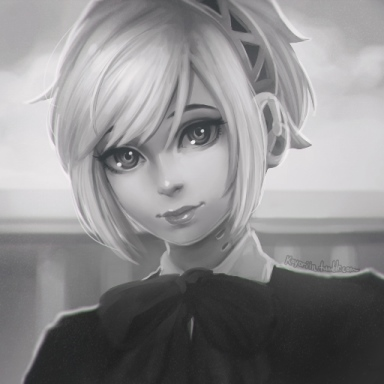
\includegraphics[scale=0.4]{grafico5.jpg}
\end{varwidth}\hfill
\begin{varwidth}{0.5\linewidth}
\begin{parts}
\item  Representa las fuerzas implicadas en cada una de las masas.
\item ¿Cuánto debe valer $m_1$, si en 2 s ha recorrido 2 m sobre el plano?
\item Calcula las tensiones de las cuerdas.
\end{parts}
\end{varwidth}
\end{minipage}
\end{problem*}
\hrule
\begin{table}[h]
\begin{center}
\begin{tabular}{|p{3.2cm}|p{1.3cm}|p{1.3cm}|p{1.3cm}|p{1.3cm}|p{1.3cm}|p{1.3cm}|}
\hline
{\scriptsize Estándar de aprendizaje}
& \centering {\scriptsize B6.2.1 \\ B6.3.1 \\ B6.6.1\\ }
& \centering {\scriptsize B6.5.1 \\ B6.8.1\\ }
& \centering {\scriptsize B6.9.2 \\ B6.9.3 \\ B6.9.4 \\ B6.9.5\\ }
& \centering {\scriptsize B7.1.1 \\ B7.2.2 \\ B7.2.3\\ }
\tabularnewline \hline {\scriptsize Preguntas o apartados \par con que se relaciona}
 &  \centering {\scriptsize 1 }
 &  \centering {\scriptsize 2 }
 &  \centering {\scriptsize 3 }
 &  \centering {\scriptsize 4 }
 \tabularnewline \hline
 {\scriptsize Puntuación máx. estándar}
  &  \centering {\scriptsize 10\\10\\10\\ } 
  &  \centering {\scriptsize 10\\20\\ } 
  &  \centering {\scriptsize 10\\10\\10\\5\\ } 
  &  \centering {\scriptsize 20\\10\\5\\ } 
\tabularnewline \hline
 {\scriptsize Puntuación obtenida } 
 &  \vspace*{1cm} \centering    \vspace*{1.5cm} 
 &  \centering  
 & \centering  
 &  \tabularnewline 
\hline 
\end{tabular}
\end{center}
\end{table}
\hrule

\hrule
\end{onehalfspace}
\end{exam} 
\end{document}
